Cykling er en aktivitetsform som udnytter kraftoverførslen mellem en person og en cykel. For at opnå en fremdrift af cyklen, benytter personen hovedsageligt en statisk position af overkroppen, hvorimod de nedre lemmer er ansvarlige for kraftudviklingen. \citep{Springer2014} \newline 
Kraftoverførslen forekommer idet personen belaster cyklens pedaler, som er påsat cyklens krank. De roterende bevægelser med de nedre ekstremiteter, skaber en fremdrift i hele systemet. Bevægelserne er opdelt i to faser, henholdsvis en kraftudøvende- og en restituerende fase, hvilket fremgår af \figref{fig:cykel_cyklus}

\begin{figure}[H]
	\centering
	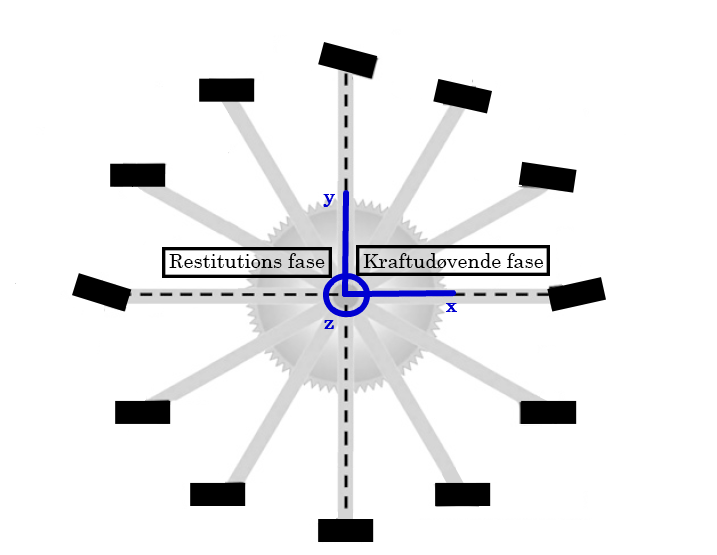
\includegraphics[scale=0.5]{figures/bProblemloesning/cykel_cyklus.png}
	\caption{XXXXX (Modificeret fra \citep{Springer2014})}
	\label{fig:cykel_cyklus}
\end{figure}
\fxnote{Opg: SKAL MODIFICERES.}

Det fremgår af ovenstående figur, at en bevægelse af de nedre ekstremiteter vil foregår om en akse. Dette pointerer andre studier ligeledes, idet disse beskriver cykling som værende en bevægelse hvor den største rotation er at finde rundt om én akse for et gyroskop. Et gyroskops datasæt vil dermed være repræsentative for den bevægelse der udføres ved cykling. \citep{Cockcroft2011,Marin-PerianuMarin-Perianu2013}
